

\documentclass[conference]{IEEEtran}
\usepackage{blindtext, graphicx}
\usepackage[utf8]{inputenc}
\usepackage[spanish, activeacute]{babel} %Definir idioma español
\usepackage{listings}
\usepackage{amssymb}
\usepackage[breaklinks=true]{hyperref}

\hyphenation{op-tical net-works semi-conduc-tor}

\begin{document}

\title{Persistencia Pol\'iglota\\Caso de estudio: MongoDB y Neo4j}

\author{
Jefferson Santiago$^{1}$, Jes\'us Ar\'evalo$^{2}$, Luinel Andrade$^{3}$\\ \\
\small{$^{1-3}$Escuela de Computaci\'on, Facultad de Ciencias}\\
\small{Universidad Central de Venezuela, 1024, Caracas, Venezuela.}\\
\small{\texttt{\{$^{1}$jefri.26.4, $^{2}$jaas1710@, $^{3}$luinel1393\}@gmail.com}} %$^{3}$lex@fechorias.com}}
}
\author{\IEEEauthorblockN{Jefferson Santiago}
\IEEEauthorblockA{Escuela de Computaci\'on\\Facultad de Ciencias\\
Universidad Central de Venezuela\\
Caracas, Venezuela\\
Email: jefri.26.4@gmail.com}
\and
\IEEEauthorblockN{Jes\'us Ar\'evalo}
\IEEEauthorblockA{Escuela de Computaci\'on\\Facultad de Ciencias\\
Universidad Central de Venezuela\\
Caracas, Venezuela\\
Email: jaas1710@gmail.com}
\and
\IEEEauthorblockN{Luinel Andrade}
\IEEEauthorblockA{Escuela de Computaci\'on\\Facultad de Ciencias\\
Universidad Central de Venezuela\\
Caracas, Venezuela\\
Email: luinel1393@gmail.com}}


% make the title area
\maketitle


\begin{abstract}
Con el auge de los sistemas de bases de datos NoSQL los cuales implementan modelos de datos diferentes al relacional como son las bases de datos documentales o de grafos, ha surgido el concepto  de Persistencia Pol\'iglota. \'Esta sostiene que debido a la gran variedad y cantidad de representación de los datos, y los diversos servicios que pueden dar las aplicaciones hoy en d\'ia; es necesario el uso de m\'as de un tipo de sistema de almacenamiento para ser capaz de cubrir de forma eficiente todas las necesidades de la aplicaci\'on que use dicho sistema.\\
En este trabajo se busca dar una idea general de las Aplicaciones de Persistencia Pol\'iglota describiendo las posibles arquitecturas  que hacen uso de las bases de datos NoSQL y su funcionamiento, se estudian algunos casos de \'exito  y se lleva a cabo un caso de estudio usando MongoDB y Neo4j.

\end{abstract}


% Note that keywords are not normally used for peerreview papers.
\begin{IEEEkeywords}
persistencia, pol\'iglota, NoSQL, MongoDB, N	eo4j.
\end{IEEEkeywords}


\IEEEpeerreviewmaketitle


\section{Introducci\'on}
En los \'ultimos a\~nos debido al uso de Internet y de nuevoas tecnolog\'ias ha aumentado la necesidad de manejar datos en vol\'umenes mayores a los que tradicionalmente manejan las bases de datos tradicionales, con 	una alta disponibilidad y escalabilidad. Es por esto que surgen las bases de datos NoSQL cuyo uso suele ser determinado por la necesidad de abarcar un fenomeno existente medi\'ante un modelo de datos apropiado, generalmente fuera del modelo relacional, sin embargo, la variedad de modelos de datos y las diferentes características t\'ecnicas entre ellas han requerido nuevos enfoques que deben establecer criterios que permitan conocer a que tareas se adaptan de forma m\'as adecuada para conseguir mejor desempe\~no y productividad.  La Persistencia Pol\'iglota se centra en el hecho de que las aplicaciones se pueden beneficiar del uso de una base de datos para cada dominio o componente de la aplicaci\'on, de esta forma aprovechar el enfoque de ”usar la mejor herramienta para el trabajo” en cada uno de los paradigmas que se necesiten contemplar, sin embargo, refiere una dificultad a nivel de integracion de las bases de datos.

\section{Modelos de datos semiestructurados}

Las bases de datos NoSQL han adoptado modelos de datos de esquema flexible que buscan adaptarse a los distintos problemas a resolver. Estos modelos se han denominado semiestructurados, debido a que aunque tienen una estructura implicita esta no es tan regular que pueda ser gestionada. 

Entre los modelos de datos semiestructurados que se han implementado se tienen
\begin{itemize}
\item \textbf{Clave valor:} Es como un mapa o diccionario, donde a una clave se le asigna un valor que puede ser cualquier estructura de datos.
\item \textbf{Familia de Columnas:} Modelo propuesto por Goggle para su base de datos BigTable \cite{BigTable} basada en el concepto de columna y la agrupación de columnas relacionadas en familias de columnas.
\item \textbf{Documentales:} Compuesto de un conjunto de tuplas clave-valor, donde el valor pueden ser datos atómicos, un arreglo u otras tuplas clave-valor. Son representados en el formato Json \cite{Json} el cual es un formato de texto para intercambio de datos estructurados entre lenguajes de programamci\'on.
\item \textbf{Grafos:} Estructura de datos donde la información se representa como nodos con propiedades y sus relaciones como enlaces \cite{neo}.
\end{itemize}

C\'omo se puede observar, cada uno de estos modelos representa la información de diferentes maneras, lo cual hace que la aplicación que use este tipo de bases de datos, tenga que adaptarse a dicha representaciones y su forma de acceso a los datos. Esto se hace m\'as complejo si la aplicaci\'on usa más de una base de datos NoSQL con modelos o formas de acceso distintos entre si. 


\section{Persistencia Pol\'iglota}


El t\'ermino Aplicaci\'on de Persistencia Pol\'iglota se basa en la idea de que las aplicaciones aprovechen las facilidades que cada modelo de datos aporta a la solución de un problema o ejecución de una tarea, que llevaría al uso de más de un sistemas de almacenamiento al la vez \cite{persistenciaPoliglota}. Lo que se busca al aplicar persistencia pol\'iglota es que las aplicaciones primero definan las tareas que van a realizar, y en base a estas, que modelo de datos se adapta mejor a las necesidades de dicha tarea. De esta forma se tendr\'an varios sistemas de bases de datos para cada aplicaci\'on. 

El principal problema a la hora de desarrollar este tipo de aplicaci\'on es manejar las distintas representaciones de los datos, dependiendo del sistema de almacenamiento, mantener las conexiones a cada base de datos y mantener la integridad entre la data. Por lo que en principio \'esto podr\'ia hacer que la aplicaci\'on fuera muy compleja. En la siguiente secci\'on se describir\'an varios diseños de arquitectura de persistencia pol\'iglota y como manejan esta complejidad.


\section{Arquitecturas de Persistencia Pol\'iglota}
Una arquitectura de persistencia políglota tiene como objetivo mostrar como se interrelacionan los diferentes elementos de persistencia políglota en un sistema o aplicación

Uno de los puntos más interesantes en las Aplicaciones de Persistencia Políglota - adem\'as
de los sistemas de almacenamiento en si - es la forma en la que se debería estructurar
la aplicaci\'on. La presencia de varios sistemas de almacenamiento trae consigo una serie
de problemas y necesidades que no existen en las aplicaciones con un \'unico sistema de
almacenamiento.

En una aplicaci\'on simple se tendr\'ia un \'unico sistema al cual se acceder\'ia para realizar las diferentes operaciones, independientemente de qu\'e tarea se trate o qu\'e datos se quieran consultar. Por tanto, la aplicaci\'on realiza operaciones que necesitan hacer diferentes consultas, pero todas ellas se hacen sobre el mismo sistema de almacenamiento como se puede observar en la figura 1

\begin{figure}[!h]
\centering
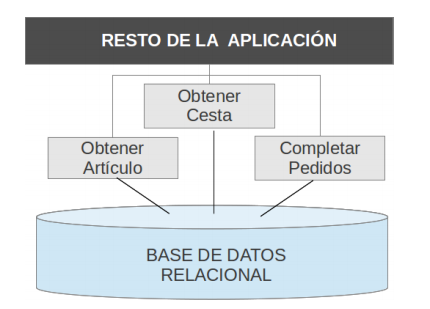
\includegraphics[width=0.4\textwidth]{1}
\caption{Ejemplo de una arquitectura con un \'unico sistema de almacenamiento.}
\label{fig1}
\end{figure}
Al introducir otros sistemas de almacenamiento, como se muestra en la figura 2, la aplicaci\'on deber\'a realizar las consultas de los datos sobre distintos sistemas, con lo que puede ocurrir lo siguiente:

\begin{itemize}
\item  No ser\'ia transparente para la aplicaci\'on el hecho de que hay m\'as de un sistema manejador actuando por debajo, por tener diferentes modelos de datos.
\item  Se deben tomar en cuenta las implicaciones que tendría agregar nuevos manejadores o realizar algún cambio en uno existente.
\end{itemize}

Un primer diseño ser\'ia el m\'as directo. En este caso, cada parte de la aplicaci\'on se comunica directamente con el sistema de almacenamiento que contiene los datos a los que se quiere acceder. Tal y como se puede ver en la figura 2 la aplicaci\'on realiza operaciones sobre cada uno de los sistemas de almacenamiento seg\'un lo vea necesario.

En principio este diseño genera varios problemas, pero uno de los principales es que la presencia de las tres bases de datos no es transparente para la aplicaci\'on, por ende, es indispensable tener conocimientos s\'olidos sobre como gestionar los datos en todos los SMBD. La problematica se presenta ya que generalmente para hacer persistencia pol\'iglota se utilizan diferentes SMBD, como en este caso, para gestionar los datos de una manera espec\'ifica para cada tarea.

\begin{figure}[!h]
\centering
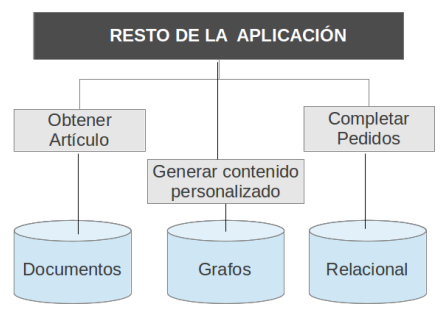
\includegraphics[width=0.4\textwidth]{2}
\caption{Arquitectura para una Aplicaci\'on de Persistencia Pol\'iglota: Diseño I.}
\label{fig2}
\end{figure}
El segundo diseño intenta eliminar los problemas anteriores. La idea es envolver las bases de datos en servicios, de forma que la aplicaci\'on no se comunique directamente con los sistemas de almacenamiento  \cite{sistemaAlmacenamiento}. \'Esta se comunicar\'a con los servicios. Estos servicios serán los encargados de realizar las consultas sobre las bases de datos. 

Con esto, por un lado se consigue que:
\begin{itemize}
\item  La distribuci\'on de los datos entre diferentes sistemas de almacenamientos sea transparente para la aplicaci\'on.

\item  Los servicios puedan ser reutilizados por otras aplicaciones que necesiten acceder a esos datos. 
\end{itemize}
Por tanto, una arquitectura con este diseño tendría forma similar al de la figura 3.

\begin{figure}[!h]
\centering
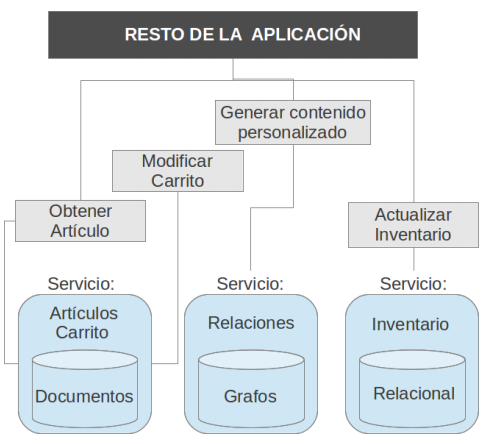
\includegraphics[width=0.4\textwidth]{3}
\caption{Arquitectura para una Aplicaci\'on de Persistencia Pol\'iglota: Diseño II.}
\label{fig3}
\end{figure}

Siguiendo la idea anterior del uso de servicios se puede considerar que hay dos posibles opciones de diseño. Por un lado, tener un servicio por cada base de datos (Figura 3) y por el otro tener servicios en funci\'on de qu\'e datos se guardan (Figura 4).

\begin{figure}[!h]
\centering
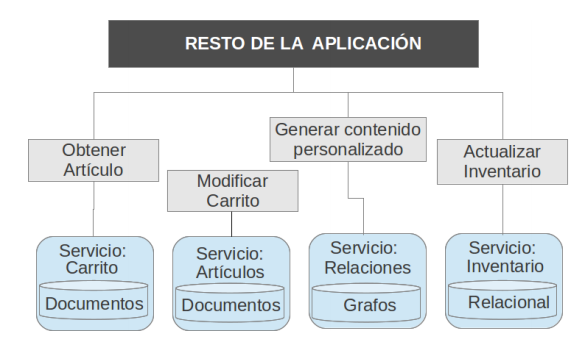
\includegraphics[width=0.5\textwidth]{4}
\caption{Arquitectura para una Aplicaci\'on de Persistencia Pol\'iglota: Diseño III.}
\label{fig4}
\end{figure}
Cualquiera de los diseños anteriores es perfectamente v\'alido, todo depende de si se tiene pensado reutilizar las consultas o se van a añadir o modificar los sistemas de bases de datos en el futuro.

\section{Casos de Exito: Wanderu y Zephyr Health}
\subsection{Wanderu}
Wanderu es una aplicaci\'on web cuya finalidad es que los consumidores puedan realizar b\'usquedas de tickets de tren y/o autob\'us, con la combinaci\'on de múltiples compañías de transporte, las rutas son almacenadas en formato JSON haciendo que la soluci\'on por excelencia trabaje con MongoDB. Sin embargo, tambi\'en tienen la opción de buscar rutas \'optimas desde un origen a un destino, tarea que es perfectamente implementable con una base de datos orientada a grafos como es el caso de Neo4J.\cite{wanderu}

Wanderu no quiso incrementar la complejidad haciendo el manejo de relaciones directamente desde MongoDB, lo que implicar\'ia mucho procesamiento y terminaria siendo ineficiente, por lo que decidieron utilizar persistencia pol\'iglota para aprovechar las bondades de ambos SMBD (MongoDB y Neo4J).

\begin{figure}[!h]
\centering
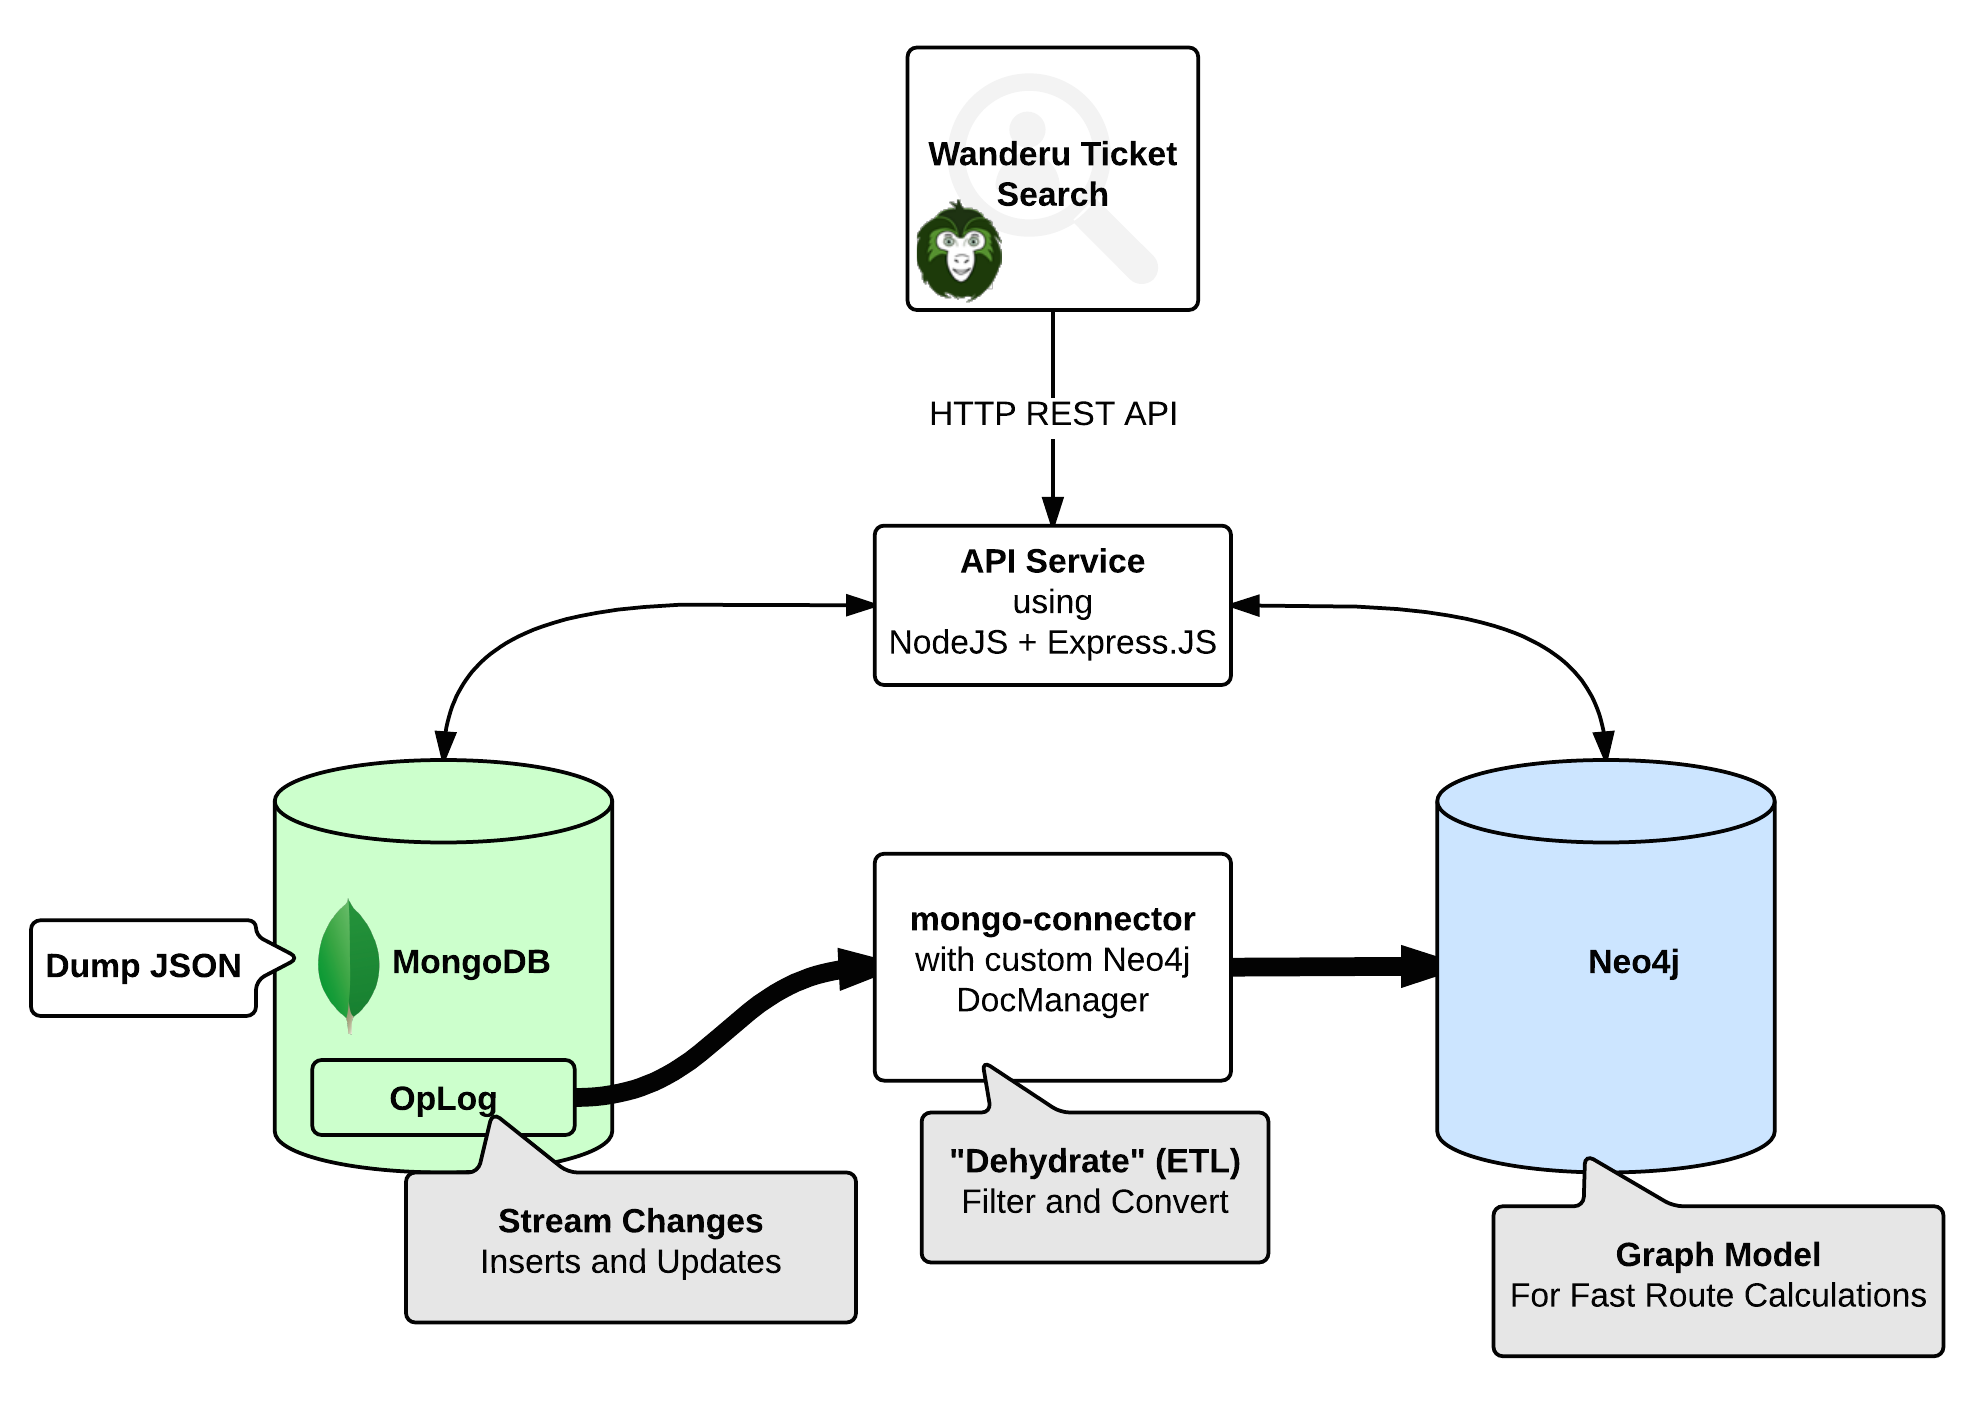
\includegraphics[width=0.4\textwidth]{wanderu}
\caption{La b\'usqueda de Wanderu utiliza MongoDB para un manejo sencillo de JSON y Neo4J para un eficiente c\'alculo de rutas}
\label{fig10}
\end{figure}

\subsection{Zephyr Health}
Zephyr Health busca integrar diversos datos de cuidado de la salud mediante el uso de MongoDB y Neo4J, su plataforma realiza complejas tareas como lo son la conexi\'on de los pacientes a los tratamientos de salud y terapias que los mismo necesitan.\cite{zephyr}

	Fundada en 2011, Zephyr Health toma data de las compañ\'ias farmac\'euticas y las transforma en informaci\'on. Permitiendo realizar an\'alisis en tiempo real que ayuda a los pacientes a conectar con diferentes terapias y tratamientos, y a las compañ\'ias farmac\'euticas a conectarse con diferentes proveedores de cuidados de la salud.

MongoDB es su almac\'en de documentos, que contiene toda la informaci\'en del perfil hol\'istico para cada m\'edico, informaci\'on de tratamientos , etc. Sin embargo el manejo de las relaciones puede ser bastante complejo al usar MongoDB, por lo que Zephyr Health decide utilizar Neo4J para solventar ciertas limitaciones de MongoDB, Neo4J es un SMBD de \'indice pesado, el rendimiento es muy coherente si se trabaja con unos pocos miles de nodos o unos pocos millones.

\section{Tecnolog\'ias Usadas}
\subsection{MongoDB}
MongoDB es una base de datos documental y \'agil de c\'odigo abierto que permite a los esquemas cambiar r\'apidamente cuando las aplicaciones evolucionan, proporcionando siempre la funcionalidad que los desarrolladores esperan de las bases de datos tradicionales, tales como \'indices secundarios, un lenguaje completo de b\'usquedas, consistencia estricta y un alto rendimiento.\cite{mongo}

\subsection{Neo4j}
Neo4j es una base de datos gr\'afica nativa altamente escalable, diseñada espec\'ificamente para aprovechar no s\'olo los datos, sino tambi\'en sus relaciones.

El motor de procesamiento y procesamiento de grafos nativo de Neo4j proporciona un rendimiento constante y en tiempo real, ayudando a las empresas a crear aplicaciones inteligentes para satisfacer los actuales desafíos de datos en constante evolución.\cite{neo}

\subsection{Neo4j Doc Manager}
Es una herramienta que permite migrar documentos desde MongoDB a una estructura de grafos de propiedades de Neo4j. Simplemente se ejecuta en segundo plano y la informaci\'on que se encuentra en MongoDB se importa a un grafo visible desde Neo4j, para permitir a los desarrolladores de MongoDB almacenar datos JSON en Mongo mientras consulta las relaciones entre los datos usando Neo4j.

MongoDB almacena datos como documentos similares a JSON, mientras que Neo4j almacena datos como grafos de propiedades. Para permitir la consulta basada en grafos de datos MongoDB, necesitamos determinar c\'omo mapear entre estas dos estructuras de datos diferentes. Neo4j Doc Manager provee un plan de mapeo por defecto. Siguiendo la convenci\'on en lugar de requerir configuraci\'on.\cite{doc}

\section{Caso de Estudio: MongoDB y Neo4j}
Al crear aplicaciones lo desarrolladores tienen una gran variedad de tecnolog\'ias para escoger, incluyendo a lo que la elecci\'on de base de datos  concierne, sin embargo, al a\~nadir nuevas tecnolog\'as a menudo termina significando mayor complejidad en el manejo de los sistemas en lugar de obtener un beneficio significante. La idea de la persistencia pol\'iglota es permitir tomar ventaja de los puntos fuertes de las distintas capas de persistencia para mejorar la funcionalidad de las aplicaciones. A continuaci\'on se presenta un caso de estudio tomado de la p\'agina oficial de Neo4j \cite{caso} basado en una aplicaci\'on de comercio electr\'onico en el que se utiliza MongoDB y Neo4j juntos en base a los puntos fuertes de cada base de datos y tambi\'en se utiliza Neo4j Doc Manager para Mongo Connector, que permite la sincronizaci\'on en tiempo real de MongoDB a Neo4j.

\begin{figure}[!h]
\centering
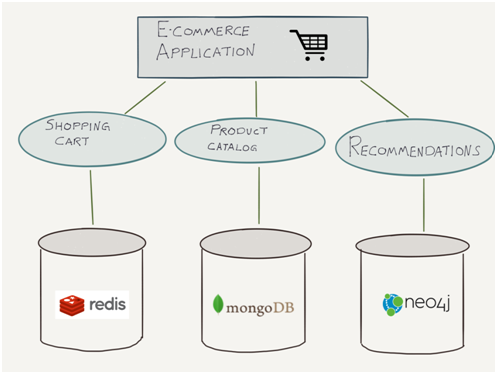
\includegraphics[width=0.4\textwidth]{5}
\caption{Se utiliza una BD claves-valor para alimentar el carrito de compras del usuario, una BD orientada a  documentos para la b\'usqueda y la navegaci\'on por el cat\'alogo de productos y una BD orientada a grafos para obtener recomendaciones personalizadas en tiempo real.}
\label{fig5}
\end{figure}

Un caso de uso b\'asico en aplicaciones de comercio electr\'onico para una base de datos documental es la de manejar un cat\'alogo de productos y poder realizar b\'usquedas sobre \'el. Entre los requisitos funcionales está el soportar una diversa cartera de productos con consultas complejas y filtrado a trav\'es de los atributos de muchos productos. Para entender c\'omo el uso de una base de datos de grafos  junto con una base de datos de documentos puede mejorar una aplicaci\'on, se tomar\'a como ejemplo una aplicaci\'on web que ofrece un cat\'alogo de cursos en l\'inea.

\begin{figure}[!h]
\centering
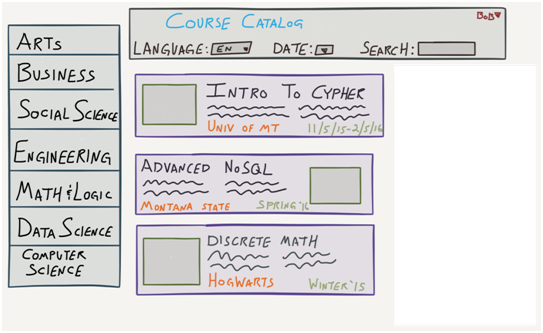
\includegraphics[width=0.5\textwidth]{6}
\caption{Un cat\'alogo de cursos en l\'inea es un buen caso de uso de una base de datos de documentos.}
\label{fig6}
\end{figure}

La vista mostrada (Figura 7) permite al usuario ver una lista de todos los cursos disponibles para ellos, buscar por palabra clave y filtrar por fecha, idioma o categor\'ia. La vista tiene que ser alimentada de una s\'ola consulta en BD por lo que se est\'a volcando una gran cantidad de informaci\'on ah\'i. Las consultas tienen que utilizar diferentes tipos de \'indices (de texto completo, filtro por categor\'ias, filtros por intervalo de tiempo) y devolver toda la informaci\'on necesaria para renderizar la vista, sin embargo, falta mostrar informaci\'on que est\'e acorde al contexto del usuario. La aplicaci\'on debe saber que cursos el usuario ha tomado anteriormente y c\'omo el usuario ha interactuado con otros usuarios en la plataforma para ser capaces de ofrecer alg\'un contenido personalizado basado en estas preferencias del usuario, por lo que entra en juego lo que ser\'ia los cursos recomendados al usuario en cuesti\'on.

\begin{figure}[!h]
\centering
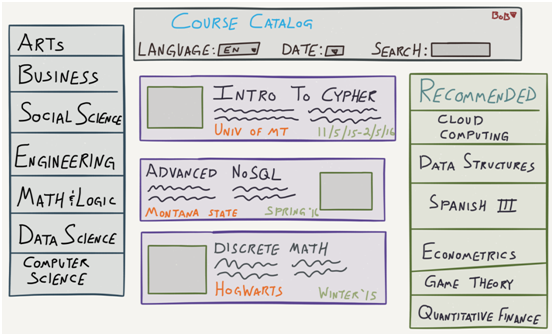
\includegraphics[width=0.5\textwidth]{7}
\caption{Cat\'alogo de cursos con contenido personalizado, tales como las recomendaciones de cursos en base a la informaci\'on que se sabe acerca de las preferencias del usuario actual.}
\label{fig7}
\end{figure}

Por sus caracter\'isticas Neo4j es muy bueno para la generaci\'on de recomendaciones en tiempo real. MongoDB podr\'ia ser la m\'as id\'onea en servir a un cat\'alogo de productos, pero si lo que se quiere es generar contenido centrado en el usuario como por ejemplo las recomendaciones personalizadas de productos se sabe que es f\'acil en Neo4j. Ahora le pregunta es ¿C\'omo?, normalmente, esto implicar\'ia la sincronizaci\'on de datos en la capa de aplicaci\'on, es decir, interactuar directamente con  MongoDB, e interactuar directamente con Neo4j pero surgen otras interrogantes como: ¿Ambas operaciones terminaron con \'exito? ¿Qu\'e hacer si una de las transacciones falla? ¿En qu\'e punto se sincronizan los datos? Esto puede convertirse r\'apidamente en un componente muy complicado. Los beneficios de la persistencia pol\'iglota se producen a expensas de la complejidad. Ahora tenemos que aplicar la l\'ogica a nivel de aplicaci\'on para escribir datos tanto MongoDB y Neo4j.

\subsection*{Neo4j Doc Manager: Habilitaci\'on de Persistencia Pol\'iglota en MongoDB y Neo4j}

El proyecto Neo4j Doc Manager de los creadores de Neo4j es una implementaci\'on del proyecto Mongo Connector, proporcionado por la gente de MongoDB. Mongo Connector proporciona un mecanismo para notificar las solicitudes y actualizaciones en MongoDB y escribir los cambios a un sistema de destino. Neo4j Doc Manager funciona mediante el uso del Oplog (un registro de todas las operaciones en MongoDB). Siempre que hay una actualizaci\'on de un documento (por ejemplo, una inserci\'on, actualizaci\'on o eliminaci\'on), Neo4j Doc Manager es notificado de la actualizaci\'on y \'este contiene la l\'ogica para convertir ese documento en un modelo de grafos con sus respectivas propiedades y, a continuaci\'on, escribe inmediatamente esa actualizaci\'on para Neo4j.

\begin{figure}[!h]
\centering
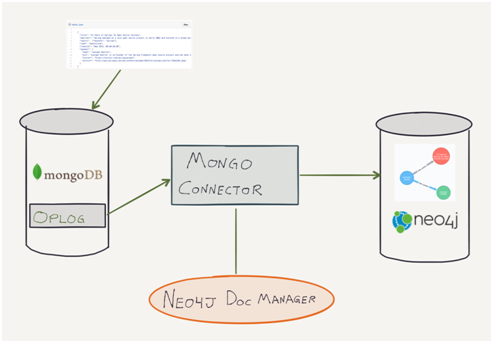
\includegraphics[width=0.5\textwidth]{8}
\caption{Neo4j Doc Manager es notificado de todas las operaciones en MongoDB, convierte esos cambios a un modelo de grafos  y de inmediato escribe esos cambios a Neo4j.}
\label{fig8}
\end{figure}

El Neo4j Doc Manager permite al desarrollador de aplicaciones alcanzar el objetivo de construir una aplicaci\'on que aprovecha la persistencia pol\'iglota con MongoDB y Neo4j. En el contexto del cat\'alogo de cursos, perfectamente se puede proporcionar b\'usqueda y navegaci\'on entre los productos con MongoDB, y proporcionar recomendaciones en tiempo real en base a lo que los cursos que el usuario ha tomado y c\'omo han interactuado con el sistema desde Neo4j.

\subsection*{Neo4j Doc Manager: Instalaci\'on e Inicio del servicio}

Ya el equipo en d\'onde se ejecutar\'a el servicio debe tener instalado y configurado MongoDB y Neo4j.\\
Se instala Neo4j Doc Manager clonando el repositorio y estableciendo el PYTHONPATH al directorio local correspondiente:

\begin{lstlisting}
git clone https://github.com/neo4j-contrib/
          neo4j_doc_manager.git
cd neo4j_doc_manager
export PYTHONPATH=.
\end{lstlisting}

Si se tiene la autenticaci\'on habilidada para Neo4j, se debe asegurar que la variable de ambiente  correspondiente contenga el nombre de usuario y la contraseña para conectarse al servidor:

\begin{lstlisting}
export NEO4J_AUTH=<user>:<password>
\end{lstlisting}

Si la autenticaci\'on est\'a deshabilitada en Neo4j esa acci\'on no es requerida. Para deshabilitar la autenticación, se tiene que ir hasta el directorio de instalaci\'on de Neo4j y editar el archivo ' conf/neo4j-server.properties'  de la siguiente manera:

\begin{lstlisting}
dbms.security.auth_enabled=false
\end{lstlisting}

Ahora, de forma adicional se debe asegurar que mongo est\'e corriendo en un conjunto de r\'eplicas. Para iniciar y establecer una réplica en Mongo basta con:

\begin{lstlisting}
mongod --replSet myDevReplSet
\end{lstlisting}

Luego, ya con el servicio iniciado, abrir una c\'onsola de Mongo y correr:

\begin{lstlisting}
rs.initiate()
\end{lstlisting}

Por \'ultimo, una vez realizado los pasos anteriores se inicia el servicio de Neo4j Doc Manager con el siguiente comando en una s\'ola l\'inea:

\begin{lstlisting}
mongo-connector -m localhost:27017 -t
http://localhost:7474/db/data -d
neo4j_doc_manager
\end{lstlisting}

-m espec\'ifica el servidor de MongoDb, -t el servidor de Neo4j (incluyendo el protocolo) y -d espec\'ifica el Neo4j Doc Manager.

\subsection*{Neo4j Doc Manager: Primeros pasos}

Los documentos se convierten en grafos en base a la estructura del documento. Las llaves del documento se convertir\'an en nodos. Los valores anidados entre cada llave se convertir\'an en propiedades.

A continuaci\'on (Figura 10) se muestra un documento que se inserta en MongoDB para ejemplificar como trabaja el Neo4j Doc Manager.

\begin{figure}[!h]
\centering
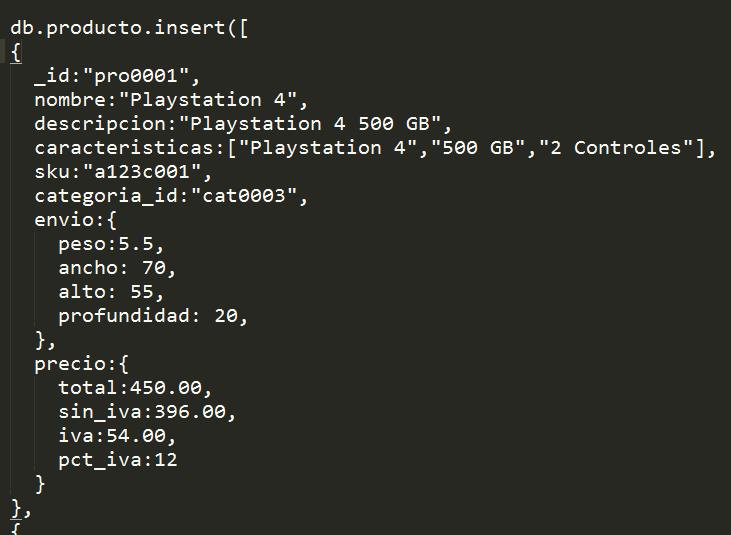
\includegraphics[width=0.5\textwidth]{10}
\caption{Documento insertado en MongoDB que se convierte a grafos en Neo4j en base a su estrcutura}
\label{}
\end{figure}

El Documento insertado en MongoDB es transformado a un modelo de grafos en Neo4j (Figura 11 y Figura 12).\\

\begin{figure}[!h]
\centering
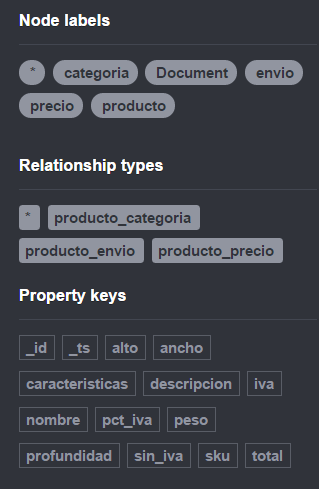
\includegraphics[width=0.3\textwidth]{11}
\caption{Informaci\'on de la base de datos en Neo4j}
\label{}
\end{figure}

\begin{figure}[!h]
\centering
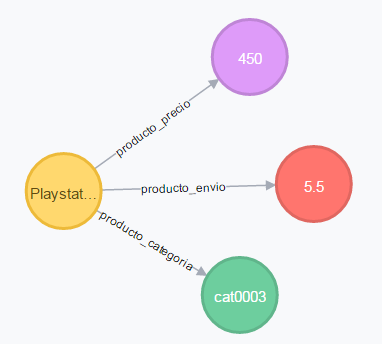
\includegraphics[width=0.45\textwidth]{12}
\caption{Grafo en Neo4j que se gener\'o seg\'un el documento insertado en MongoDB}
\label{}
\end{figure}

Nodos creados:\\
\begin{itemize}
\item producto: producto es el nodo ra\'iz, viene del nombre de la colecci\'on a la que pertenece el documento con un  ''\_id'' que tambi\'en viene de MongoDB. Documentos no anidados son convertidos a propiedades del nodo, como por ejemplo: ''nombre'',''descripcion'', ''caracteristicas'',''sku'.
\item envio: envio es un documnto embebido. Pares claves-valor que est\'en dentro son convertidos a propiedades del nodo como por ejemplo: ''peso'', ''ancho'', ''alto'', ''profundidad''. Tambi\'en tiene una propiedad ''\_id'' que viene del nodo ra\'iz y es la mismo.
\item precio: precio es un documento embebido por lo que es análogo al nodo session.
\item categoria: en la colecci\'on producto hay una clave ''categoria\_id'' que Neo4j Doc Manager toma como una referencia a un nodo con etiqueta categoria que contenga ese id y crea la relaci\'on entre ellos. En caso de no existir, crea el nodo categoria y le asigna el id que tiene como valor en el documento.
\end{itemize}
También es importante mencionar que a los nodos se les agrega autom\'aticamente una propieda ''\_ts'' que representa su timestamp de la creaci\'on en MongoDB.\\

Relaciones creadas:\\

\begin{itemize}
\item producto\_precio: Una relaci\'on que conecta a los nodos producto y precio.
\item producto\_envio: Una relaci\'on que conecta a los nodos producto y envio.
\item producto\_categoria: Una relaci\'on que conecta a los nodos producto y categoria.\\
\end{itemize}

Ya visto como se hace la conversi\'on de un documento en MongoDB a grafos en Neo4j podr\'ia decirse que las posibilidades son muchas, ya que desde MongoDB se puede trabajar directamente con las colecciones y los datos se ver\'an reflejados en Neo4j para despu\'es procesar consultas relacionas a estructuras de grafos. Desde Mongo se puede hacer actualizaciones y eliminaciones  seg\'un criterios de filtrado que se reflejar\'an en Neo4j y que permitir\'an hacer cosas como por ejemplo: agregar o eliminar propiedades en los nodos, cambiar la estructura de los mismos, agregar o eliminar relaciones, entre otras cosas. Para ello, se invita al lector a profundizar m\'as en el tutorial de Neo4j Doc Manager que se encuentra en la p\'agina oficial de Neo4j  y en donde se explica de manera detallada los comandos a ingresar en MongoDb y los resultados obtenidos. Tutorial disponible en el siguiente enlace:\\
\url{https://neo4j.com/developer/neo4j-doc-manager/}

\subsection*{Neo4j Doc Manager: Aplicaci\'on de Persistencia Pol\'iglota}

Siguiendo el esquema propuesto (Figura 6) para una aplicaci\'on de persistencia pol\'iglota  los autores del presente documento desarrollar\'on una sencilla aplicaci\'on de comercio electr\'onico (Figura 13) que maneja datos provenientes de diferentes sistemas manejadores de base de datos para su funcionamiento.

\begin{figure}[!h]
\centering
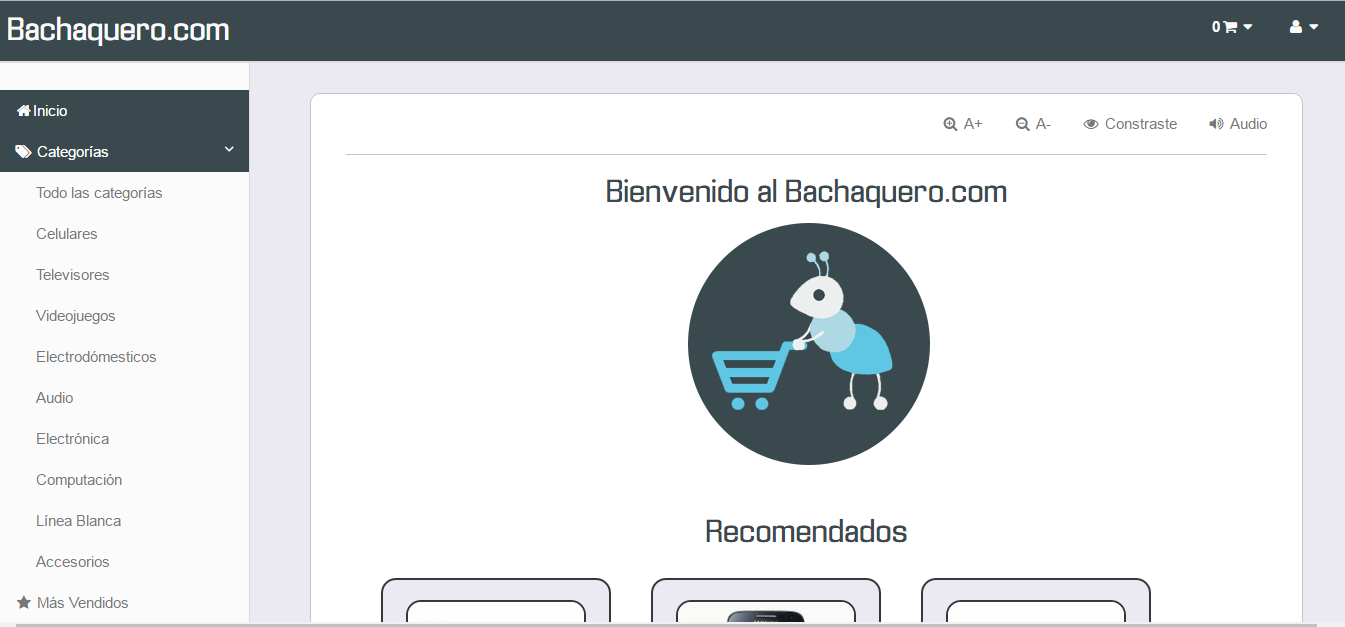
\includegraphics[width=0.5\textwidth]{13}
\caption{Vista general de la aplicaci\'on de comercio electr\'onico}
\label{}
\end{figure}

Las secciones de categor\'ias y de cat\'alogo de productos (Figura 14) se alimentan de datos almacenados en MongoDB. Se muestra contenido adecuado al contexto del usuario mediante recomendaciones (Figura 15) que se hacen a trav\'es de consultas hechas en Neo4j y se cuenta con un carrito de compras (Figura 16) que se puede implementar mediante una base de datos clave-valor.

\begin{figure}[!h]
\centering
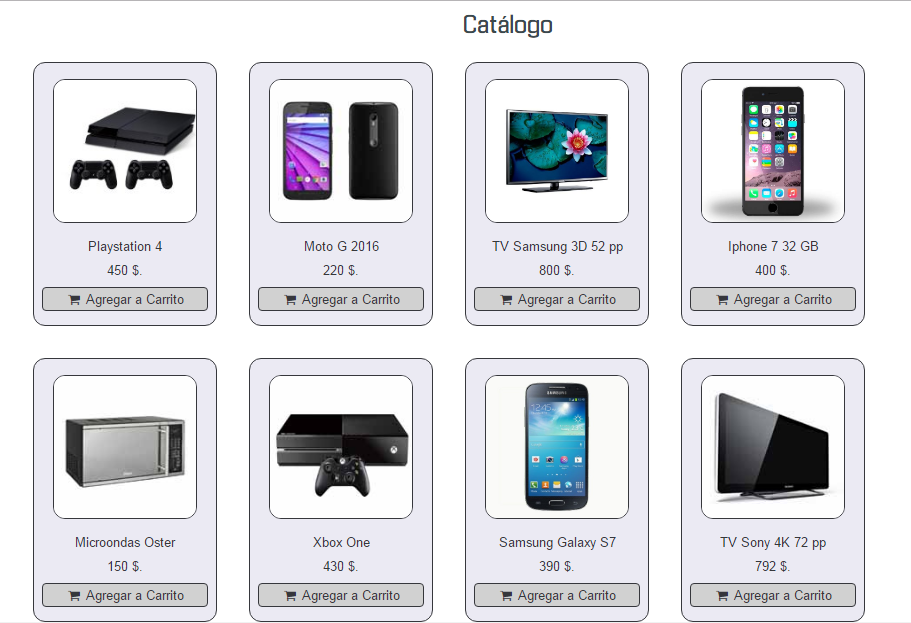
\includegraphics[width=0.5\textwidth]{14}
\caption{Cat\'alogo de productos de la aplicaci\'on de comercio electr\'onico con datos obtenidos de MongoDB}
\label{}
\end{figure}

\begin{figure}[!h]
\centering
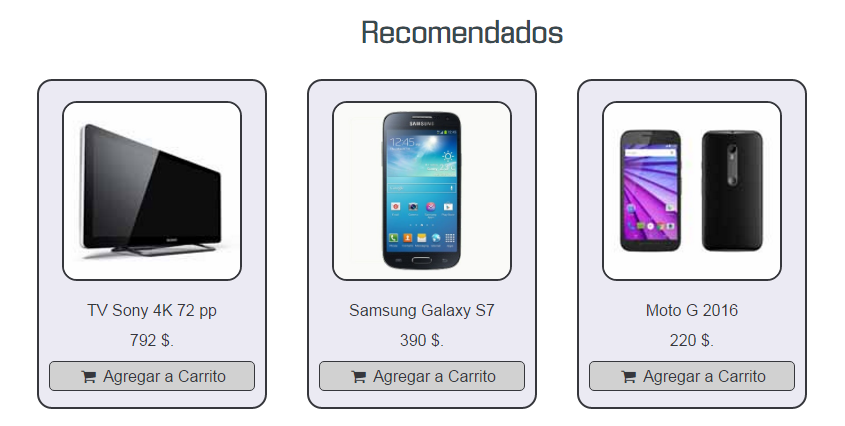
\includegraphics[width=0.5\textwidth]{15}
\caption{Productos recomendados al usuario en la aplicaci\'on de comercio electr\'onico con datos obtenidos de Neo4j}
\label{}
\end{figure}

\begin{figure}[!h]
\centering
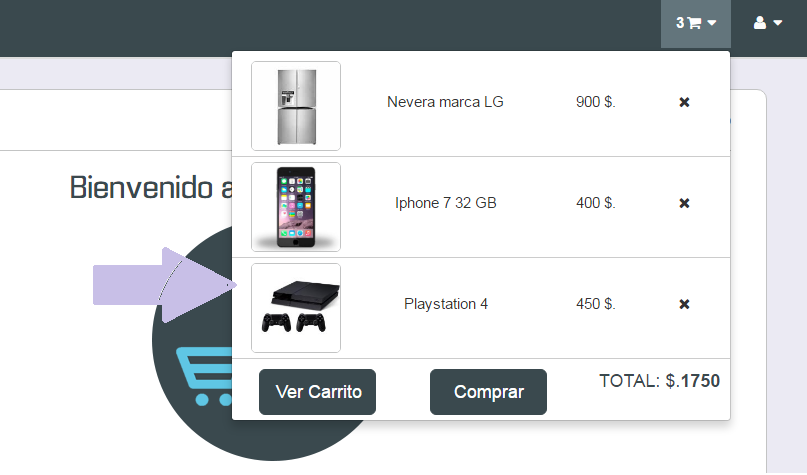
\includegraphics[width=0.45\textwidth]{16}
\caption{Carrito de compras de la aplicaci\'on de comercio electr\'onico}
\label{}
\end{figure}


\section{Conclusiones}
  Cuando se trata de construir aplicaciones escalables, los desarrolladores poseen un millar de tecnologias de donde escoger, especialmente cuando se trata de la elecci\'on de SMBD. Lo que se busca es escoger las tecnolog\'ias adecuadas que ofrezcan las funcionalidades necesarias bajo un desempeño ideal.

  La idea de la persistencia pol\'iglota permite tomar ventajas sobre las diferentes cosas que nos ofrecen los SMBD al mismo tiempo para tener aplicaciones escalables. 

  Teniendo todo esto en cuenta la pregunta que hay que hacerse es ¿merece la pena hacer una Aplicaci\'on de Persistencia Pol\'iglota? La respuesta es que depende. En una aplicaci\'on simple y con poca carga de datos, la realidad es que un \'unico sistema es más que suficiente. Sin embargo, en una aplicaci\'on con muchos datos de diferente tipo y con diferentes necesidades se puede sacar provecho del uso de varios sistemas frente a uno solo donde el rendimiento baje o la complejidad del esquema de datos desborde al desarrollador y a los administradores.


% Can use something like this to put references on a page
% by themselves when using endfloat and the captionsoff option.
\ifCLASSOPTIONcaptionsoff
  \newpage
\fi



% trigger a \newpage just before the given reference
% number - used to balance the columns on the last page
% adjust value as needed - may need to be readjusted if
% the document is modified later
%\IEEEtriggeratref{8}
% The "triggered" command can be changed if desired:
%\IEEEtriggercmd{\enlargethispage{-5in}}

% references section

% can use a bibliography generated by BibTeX as a .bbl file
% BibTeX documentation can be easily obtained at:
% http://www.ctan.org/tex-archive/biblio/bibtex/contrib/doc/
% The IEEEtran BibTeX style support page is at:
% http://www.michaelshell.org/tex/ieeetran/bibtex/
%\bibliographystyle{IEEEtran}
% argument is your BibTeX string definitions and bibliography database(s)
%\bibliography{IEEEabrv,../bib/paper}
%
% <OR> manually copy in the resultant .bbl file
% set second argument of \begin to the number of references
% (used to reserve space for the reference number labels box)
\begin{thebibliography}{1}

\bibitem{persistenciaPoliglota}
Guti\'errez E. Aplicaci\'on de Persistencia Pol\'iglota para Almacenamientos NoSQL.Universidad del Pais Vasco, 2016.

\bibitem{sistemaAlmacenamiento}
Pramod J. Sadalage Martin Fowler. NoSQL Distilled: A brief Guide to the Emerging
World of Polyglot Persistence. Addison-Wesley, 2013.

\bibitem{BigTable}
Fay Chang, Jeffrey Dean, Sanjay Ghemawat, Wilson C. Hsieh, Deborah A. Wallach, Mike Burrows, Tushar Chandra, Andrew Fikes, and Robert E. Gruber. 2008. Bigtable: A Distributed Storage System for Structured Data. ACM Trans. Comput. Syst. 26, 2, Article 4 (June 2008), 26 pages. DOI=http://dx.doi.org/10.1145/1365815.1365816

\bibitem{NoSQL}
Vaish, Gaurav. Getting Started with NoSQL. Packt Publishing, 2013.

\bibitem{Json}
ECMA-404. Introducción a JSON. 2013. [online]
Disponible en: http://www.json.org/json-es.html

\bibitem{wanderu}
Boyd R. Polyglot Persistence Case Study: Wanderu + Neo4j + MongoDB Neo4j Blog, 2015.

\bibitem{zephyr}
Chaudhari M. Integrating Diverse Healthcare Data using MongoDB and Neo4j.Neo4j Blog, 2016.

\bibitem{mongo}
MongoDB, Inc. Reinventando la gestión de datos. [online]
Disponible en: https://www.mongodb.com/es

\bibitem{neo}
Neo Technology, Inc. Neo4j: The World’s Leading Graph Database. [online]
Disponible en: https://neo4j.com/product/

\bibitem{doc}
Neo Technology, Inc. Neo4j: The World’s Leading Graph Database. [online]
Disponible en: https://neo4j.com/developer/neo4j-doc-manager/

\bibitem{caso}
Lyion W. Neo4j Doc Manager: Polyglot Persistence for MongoDB and Neo4j. Neo4j Blog, 2015.

\end{thebibliography}

\begin{IEEEbiography}[{\includegraphics[width=1in,height=1.25in,clip,keepaspectratio]{picture}}]{John Doe}
\blindtext
\end{IEEEbiography}



\end{document}


